\documentclass{article}
\usepackage{amssymb,amsmath,graphicx,color,multicol,mycommands}
\usepackage{amsfonts}
\usepackage{algorithm,url}
\usepackage[noend]{algpseudocode}
\usepackage{epsfig,latexsym,graphicx}
\parindent 0in

\title{Weighted Projection Quantiles Algorithm}


\begin{document}
\maketitle

\paragraph{Algorithm to calculate weighted projection quantile} along the vector $\bfu \in\mathcal B_p$, given a set of observations $\bfX_1,\bfX_2,...,\bfX_n$:

\begin{enumerate}

\item \textbf{\textit{Compute $Q_{proj}(\bfu)$, the projection quantile along $\bfu$}}

\begin{itemize}
\item Project each $\bfX_i$ along $\bfu$ to obtain $X_{\bfu i}=\frac{\langle\bfX_i,\bfu\rangle}{\|\bfu\|}$, for $i=1,2,...,n$.
\item Find $\alpha=\frac{1+\|\bfu\|}{2}$-th quantile of $X_{\bfu 1},...,X_{\bfu n}$, say $q_\bfu$..
\item $Q_{proj}(\bfu)=q_\bfu\bfe_\bfu$, $\bfe_\bfu=\bfu/\|\bfu\|$ being the unit vector along $\bfu$.

\end{itemize}

\item \textit{\textbf{Compute Weights corresponding to this projection quantile $Q_{proj}(\bfu)$}}

\begin{itemize}

\item Compute global weights for the direction vector $\bfu$ by $k$-mean distance:

\begin{itemize}
\item Compute $k$-mean distance corresponding to $Q_{proj}(\bfu)$ using $\bar d_k=\frac{1}{n}\sum_{i=1}^nd_i\mathbb{I}_{\{d_i<d_{(k)}\}}$, where $d_i$ is the euclidean distace of $\bfX_i$ from $Q_{proj}(\bfu)$ given by $\|\bfX_i-Q_{proj}(\bfu)\|$. $k$ is a tuning parameter.\\

\item Compute the weights corresponding to $\bfu$:
$$w_\bfu=\exp(-a.d_k)$$
where $a$ is a tuning parameter. 
\end{itemize}

\item Compute weights for each sample point $\bfX_i; i=1,2,...,n$:

\begin{itemize}
\item Compute the orthogonal Norms by $\|\bfX_{\bfu\perp i}\|=\|\bfX_i-X_{\bfu i}\bfe_\bfu\|$.

\item Compute weight of $i^{th}$ sample:
$$w_{2i} = \exp\left[-b\frac{\|\bfX_{\bfu\perp i}\|}{\|\bfX_i\|}\right]\mathbb{I}_{\{\|\bfX_{\bfu\perp i}\|\leq\epsilon\}}$$
$b,\epsilon$ being tuning parameters.
\end{itemize}
\end{itemize} 

\item \textit{\textbf{Compute the weighted projection quantile}}
\begin{itemize}
\item Suppose there are $m$ observations with non-zero weights $w_{2i}$, with indices $i_1,i_2,...,i_m$. Define $\tilde X_{\bfu i_j} = w_\bfu w_{2i_j}X_{\bfu i_j}$.
\item Find $\alpha=\frac{1+\|\bfu\|}{2}$-th quantile of $\tilde X_{\bfu i_1},...,\tilde X_{\bfu i_m}$. Let it be $\tilde q_\bfu$.
\item Find the weighted projection quantile as $\tilde Q_{proj}(\bfu)=\tilde q_\bfu\bfe_\bfu$.
\end{itemize}
\end{enumerate}
\newpage

\paragraph{Definition} Given a random vector $\bfX\in \mathbb{R}^p$ that follows a multivariate distribution $F$, and a point $\bfp\in\mathbb{R}^p$, find $\alpha_\bfp$ such that $\|\bfp\|$ is the $\alpha_\bfp$-th quantile for the projection of $\bfX$ on $\bfp$, say $X_\bfp$. Then the \textbf{Projection Quantile Depth} (PQD) at $\bfp$ with respect to $F$ is defined as
$$ D(\bfp, F) = \exp(-\alpha_\bfp) $$

\paragraph{} Given data $\bfX_1,\bfX_2,...,\bfX_n$, the PQD at a given $\bfp$ can be estimated by finding the two nearest points on either side of $\|\bfp\|$ along $\bfp$, say $\bfp_1, \bfp_2$, obtain their corresponding quantiles, say $\alpha_1, \alpha_2$ respectively, then estimate $\alpha_\bfp$ by a linear approximation:
$$\hat\alpha_\bfp=\frac{(\alpha_1-\alpha_2)(\|\bfp\|-\|\bfp_1\|)}{\|\bfp_1\|-\|\bfp_2\|}+\alpha_1$$
and plugging it in the above definition.

\begin{algorithm}[h]
\caption{Algorithm for PQD-based classification}
\begin{algorithmic}[1]
\Procedure{PQDClassifier}{training data $\bfX_i \in\mathbb{R}^{n_i\times p}$ with class labels $i$; $i=1,2,...,k$, new data $\bfx_{new}\in\mathbb{R}^p$}
\State Set $i=1$.
\State \emph{top}:
\State Estimate from the sample the PQD of $\bfp$ with respect to the $i^{th}$ population, say $D(\bfx_{new},\bfX_i)$.
\If {$i=k$} \textbf{Stop}
	\Else \State Set $i\leftarrow i+1$, \textbf{goto} \emph{top}
\EndIf
\\
\State Find $c$ that maximizes the PQD of $\bfx_{new}$ w.r.t. all possible classes:
$$ D(\bfx_{new},\bfX_c) = \max\{D(\bfx_{new},\bfX_i): i=1,2,...,k\} $$
\State Assign class $c$ to new data $\bfx_{new}$.

\EndProcedure
\end{algorithmic}
\end{algorithm}

\paragraph{Note} One can define a weighted version of PQD by replacing $X_\bfp$ by their weighted version $\tilde X_\bfp$. A weighted classification scheme follows similarly.

%\section*{Modifications}
%\paragraph{1. $w_{2i}=\mathbb{I}_{\{\|X_{\bfu\perp i}\|\leq\epsilon\}}$}
%Wouldn't work. The objective function here is
%\begin{eqnarray*}
%\tilde\Psi_\bfu(q) &=& \mathbb{E}\left[\lbrace |X_\bfu-q|+\alpha(X_\bfu-q)\rbrace\mathbb{I}_{\{\|\bfX_{\bfu\perp}\|\leq\epsilon\}}\right]\\
%&=&\mathbb{E}\left[|X_\bfu-q|+\alpha(X_\bfu-q)\right]P\left[\|\bfX_{\bfu\perp}\|\leq\epsilon\right]\\
%&=&\Psi_\bfu(q)P\left[\|\bfX_{\bfu\perp}\|\leq\epsilon\right]
%\end{eqnarray*}
%because $Cov(X_\bfu\bfe_\bfu,\bfX_{\bfu\perp})=\bf{0}$. Hence it gives out PQ as the minimizer.

\section*{New notion of data depth}We define a data depth based on projection quantiles (which, of course, can be extended to the weighted versions), on the lines of Zuo's Projection Depth [ref?].
\paragraph{Definition}
Given a random vector $X\in \mathbb{R}^p$ that follows a multivariate distribution $F$, and a point $x\in\mathbb{R}^p$, define an outlyingness function
$$ O(x,F) = \sup_{\|u\|=1} \left\vert F_u(x_u)-\frac{1}{2}\right\vert $$
where $F_\bfu$ is the distribution function of $X_\bfu$, and $x_u=\langle x,u\rangle/\|u\| $. Then we define the \textbf{Projection Quantile Depth} at $x$ with respect to $F$ as
$$ PQD(x,F) = \frac{1}{1+O(x,F)} $$

\paragraph{}We now follow the order in Zuo's paper to obtain the properties of the PQD.

\paragraph{(P1) \textit{Affine invariance}} Say $G$ is the cdf of $AX+b$. Then we have $O(Ax+b,G)=O(x,F)$ because for all $u\in\mathbb{R}^p$ we have
$$ F(x)= G(Ax+b) \Rightarrow F_u(x_u) = G_{Au+b}\left((Ax+b)_{Au+b}\right)$$
where subscripting denotes projection.

\paragraph{(P2) \textit{Quasi-concavity}} for $0<\lambda<1, z=\lambda x+(1-\lambda)y$,
\begin{eqnarray*}
F_u(z_u) &=& F_\bfu (\lambda x_u+(1-\lambda)y_u)\\
\Rightarrow \left\vert F_u(z_u)-\frac{1}{2}\right\vert &\leq &
\begin{cases}
\left\vert \max\{F_u(x_u),F_u(y_u)\}-\frac{1}{2}\right\vert & \mbox{if } F_u(z_u)<1/2\\
\left\vert \min\{F_u(x_u),F_u(y_u)\}-\frac{1}{2}\right\vert & \mbox{otherwise}
\end{cases}\\
&\leq & \max\left\lbrace \left\vert F_u(x_u)-\frac{1}{2}\right\vert, \left\vert F_u(y_u)-\frac{1}{2}\right\vert \right\rbrace
\end{eqnarray*}
and we finally get $PQD(z,F)\geq\max\{PQD(x,F),PQD(y,F)\}$.

\paragraph{(P3) \textit{Vanishing at infinity}}For $\|x\|\rightarrow\infty$ we have $F_u(x_u)\rightarrow 1$ hence $PQD(x,F)\rightarrow 2/3$. So we can define $PQD^*(x,F)=PQD(x,F)-2/3$ to obtain P3.

\paragraph{(P4) \textit{Maximized at center of symmetric $F$}} Halfspace symmetry of $F$ w.r.t. center $\theta$ implies (halfspace) symmetry of $F_u$ around $\theta_u$ for any $u\in\mathbb{R}^p$, so that $F_u(\theta_u)=1/2$ and subsequently $PQD$ achieves its max value 1 at $\theta$.

\paragraph{Example 1}For $X\sim \mathcal{N}_2((0,0)',I_2)$ we have $X_u\sim N(0,1)$ for any $u\in\mathbb{R}^p: \|u\|=1$. Due to the symmetry of the distribution function maximizing $|F_u(x_u)-1/2|$ is equivalent to maximizing $F_u(x_u)=\Phi(x_u) = \Phi(\langle x,u\rangle)$.

\paragraph{} Converting $u$ to polar coordinates we can maximize over the angle $\theta$ that $u$ makes with the X-axis, and can easily find that the above function maximizes at $\theta = \tan^{-1}(x_2/x_1)$, which is the direction for $x$ itself. Thus for given $x$ the sup is obtained at $u=x$, and we have
\begin{equation}
PQD(x,F) = \frac{1}{1+\Phi(\|x\|)-1/2} = \frac{2}{1+2\Phi(\|x\|)}
\end{equation}

Fig. 1 shows a comparison of PQD with Zuo's PD for standard bivariate normal.
%\begin{figure}[t]
%	\centering
%		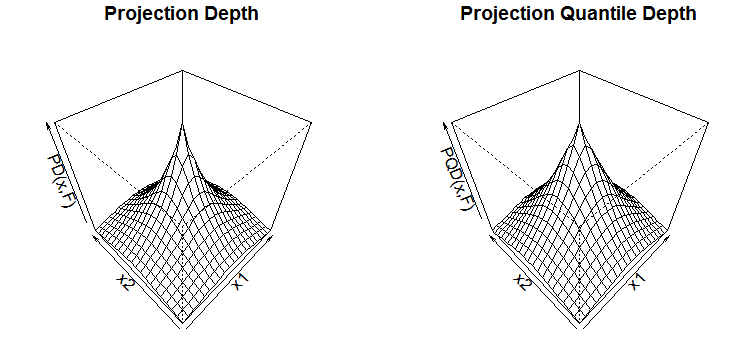
\includegraphics[height=4cm]{pd_vs_pqd_bvn3d.png}\\
%	\label{fig:fig1}
%	\caption{Projection Depth (left) and Projection Quantile Depth (right) for $\mathcal{N}_2((0,0)',I_2)$}
%\end{figure}
\paragraph{Note} In place of standard bivariate normal, one can use any circularly symmetric $F$, i.e. a distribution that has the same marginal distribution $F_0$ along all one-dimensional projections to come up with an exact formula for $PQD(x,F)$. In that general scenario, $\Phi(.)$ will be replaced by $F_0(.)$ in (1).

\section*{A general class of projection based depth functions}
\paragraph{Definition}
We consider a random variable $X\in\mathbb{R}^p$ following the distribution $F$. Define $F_u$ as the projection of $F$ towards any $u\in\mathbb{R}^p$. In this setup, we define a general class of outlyingness (or htped) function:
\begin{eqnarray}
O(x,F) = \sup_{\|u\|=1} f(x_u,\theta(F_u))
\end{eqnarray}

where $f(.)$ is a function satisfying properties mentioned below. $x_u=\langle x,u\rangle/\|u\| $, and $\theta(F_u)$ is a set of parameters (or a parameter) characterizing the distribution function $F_u$. Then we define the depth at $x$ with respect to $F$ as $ D(x,F) = 1/(1+O(x,F)) $.

The necessary properties of $f(.)$ are formulated keeping necessary properties of a depth functions in mind [ref zuo-serf]:
\paragraph{(F1) \textit{Affine invariant}} $f(x_u,\theta_u) = f(Ax_u+b,\theta^{AX+b}_u)$ for non-singular matrix $A\in\mathbb{R}^{p\times p}$.
where subscripting denotes projection.

\paragraph{(F2) \textit{Quasi-convex in $x_u$}} for $0<\lambda<1, z=\lambda x+(1-\lambda)y$,
$$ f(z_u) = f(\lambda x_u+(1-\lambda)y_u) \leq \max\lbrace f(x_u,\theta_u), f(y_u,\theta_u)\rbrace$$
from which quasi-concavity of $D(x,F)$ follows.

\paragraph{(F3) \textit{Monotonically increasing in $x_u$}} ???

\paragraph{(F4) \textit{Maximized at center of symmetric $F$}} ??

\paragraph{(F5) \textit{Uniformly continuous in both $x_u$ and $\theta(F_u)$}}

\paragraph{Theorem 0} Given an outlyingness function like (1) and an $f(.)$ satisfying properties (F1)-(F5), the resulting depth function is:
\begin{enumerate}
\item Affine invariant,

\item Quasi-concave, and as a result $D(x,F)$ decreases monotonically along any ray starting from the deepest point, [ref]

\item Maximized at the center of a symmetric $F$.

\item Uniformly continuous.
\end{enumerate}
The proofs easily follow from the corresponding properties of $f(.)$.

\paragraph{}Now suppose that $\theta_{nu}$ is the estimate of $\theta_u$ from a size-$n$ iid sample. Following Zuo, we state some properties regarding the convergence $\theta_{nu}\rightarrow\theta_u$.

\paragraph{(C0)} $ \sup_{\|u\|=1} |\theta_i(F_u)| < \infty$ for $i=1,2,...,k$.

\paragraph{(C1)} $ \sup_{\|u\|=1} |\theta_i(F_{nu})-\theta_i(F_u)| = o_P(1)$ for $i=1,2,...,k$.

\paragraph{(C2)} $ \sup_{\|u\|=1} |\theta_i(F_{nu})-\theta_i(F_u)| = o(1)$ a.s. for $i=1,2,...,k$.

\paragraph{(C3)} $ \sup_{\|u\|=1} |\theta_i(F_{nu})-\theta_i(F_u)| = O_P(1/\sqrt n)$ for $i=1,2,...,k$.

\end{document}